\section{End-to-End Transfers}
All of the transfers used in this investigation arrive into the same Sun-Mars northern halo orbit
($JC=3.0001857$) using the smallest periapsis stable manifold as the MMAT example in
\cref{fig:MMATSM}. The end-to-end methodology for constructing both categories of transfers is as
follows:

\subsection{Transfers with "Direct" System Departure}
\begin{enumerate}
    \item   Starting from the Earth-Moon CR3BP departure orbit, both unstable half-manifolds are
            propagated to the edge of the Earth's SoI (ignoring those that crash into the Earth or
            Moon), where they are transformed into heliocentric inertial states and propagated
            under Keplerian dynamics. This is repeated for several different epochs during January
            2026.
    \item   Each of these feasible manifold arcs then serves as a departure CR3BP arc and departure
            conic arc for the MMAT methodology introduced in Section 4.2. If they meet the MMAT\
            inequality constraint (\cref{eq:MMAT}), then they produce two end-to-end "direct"
            transfers between an Earth-Moon and Sun-Mars orbit.
\end{enumerate}

This transfer type is denoted as "direct" since it directly departs from the system along the
invariant manifold arc instead of using a staging orbit, not to be confused with direct patched
conic transfers between the Earth and Mars. An example "direct" transfer is shown in
\cref{fig:directE} and \cref{fig:directMMAT}. The departure CR3BP arc originates from an Earth-Moon
northern $L_{2}$ halo with a Jacobi constant of $3.13$ in \cref{fig:directE}(a), shown in the
Earth-Moon rotating frame, and continues under the Sun-Earth dynamics until it reaches the Earth
SoI in \cref{fig:directE}(b).

Note that this trajectory is not optimized, nor is it the minimum-TOF or minimum-$\Delta v$
solution in the MMAT family originating from that Earth-Moon departure orbit. This particular
"direct" transfer has a total maneuver cost of $5.544$ km/s with a total time-of-flight of $3.26$
years.

\begin{figure}[ht]
    \begin{subfigure}[h]{0.495\linewidth}
        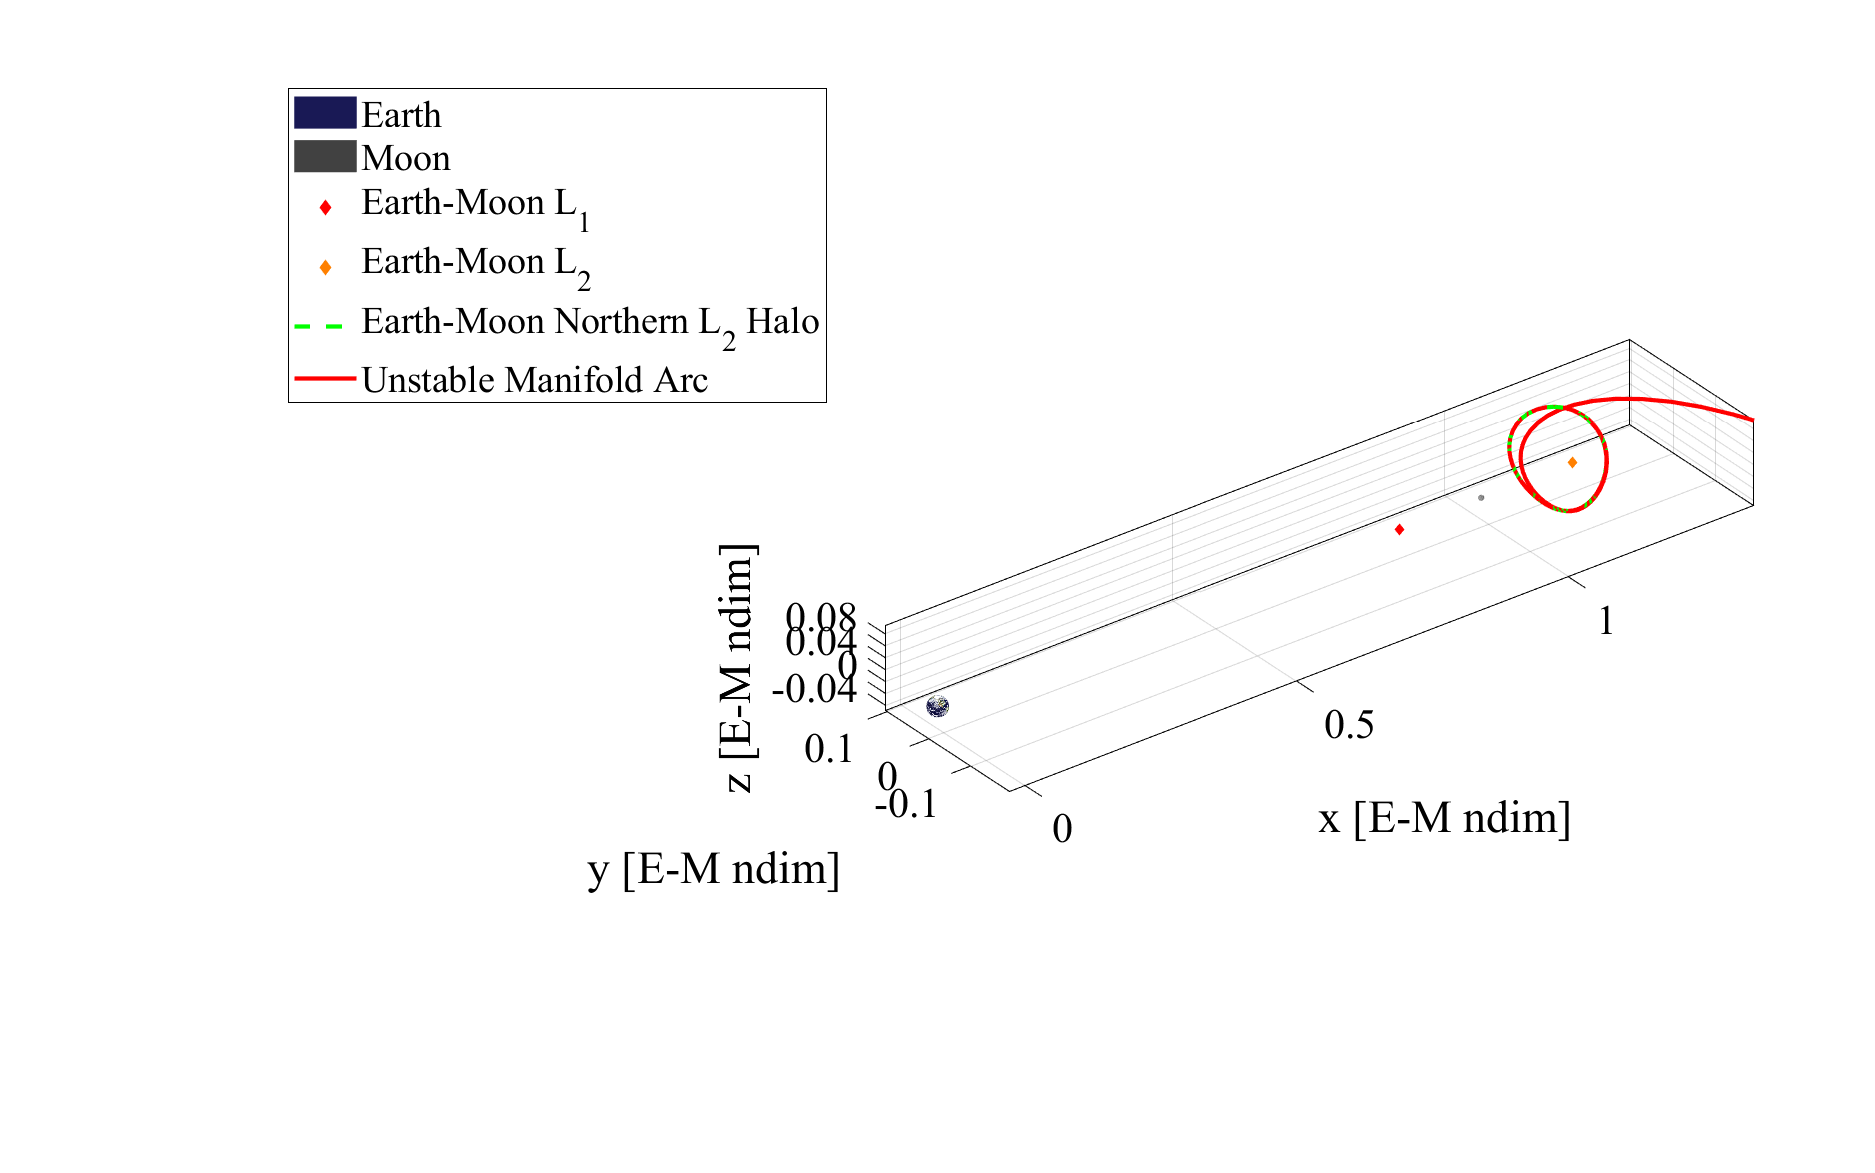
\includegraphics[width=\textwidth]{figures/DirectEM.pdf}
        \caption{Earth-Moon barycentric rotating frame.}
    \end{subfigure}
    \hfill
    \begin{subfigure}[h]{0.495\linewidth}
        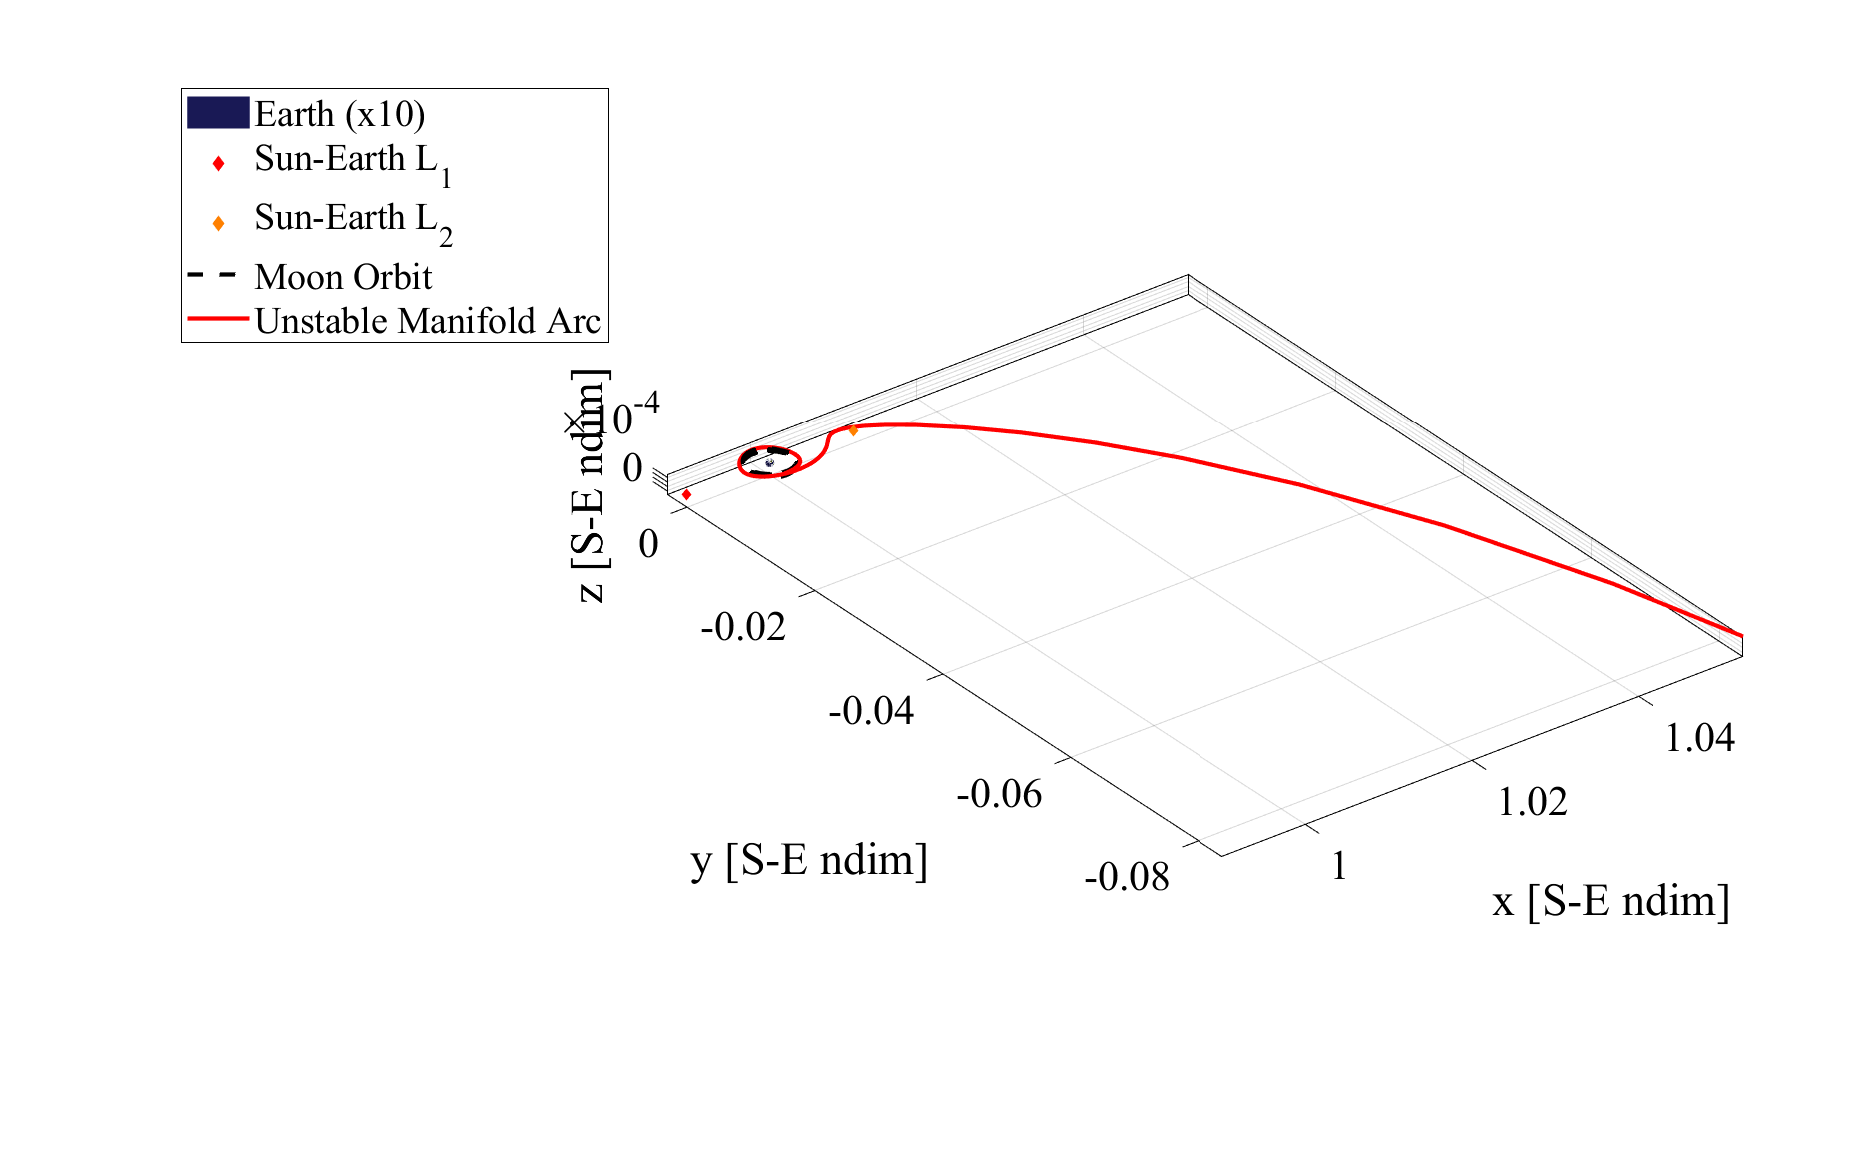
\includegraphics[width=\textwidth]{figures/DirectSE.pdf}
        \caption{Sun-Earth barycentric rotating frame.}
    \end{subfigure}
    \caption{"Direct" departure CR3BP arc.}
    \label{fig:directE}
\end{figure}

\begin{figure}[ht]
    \centering
    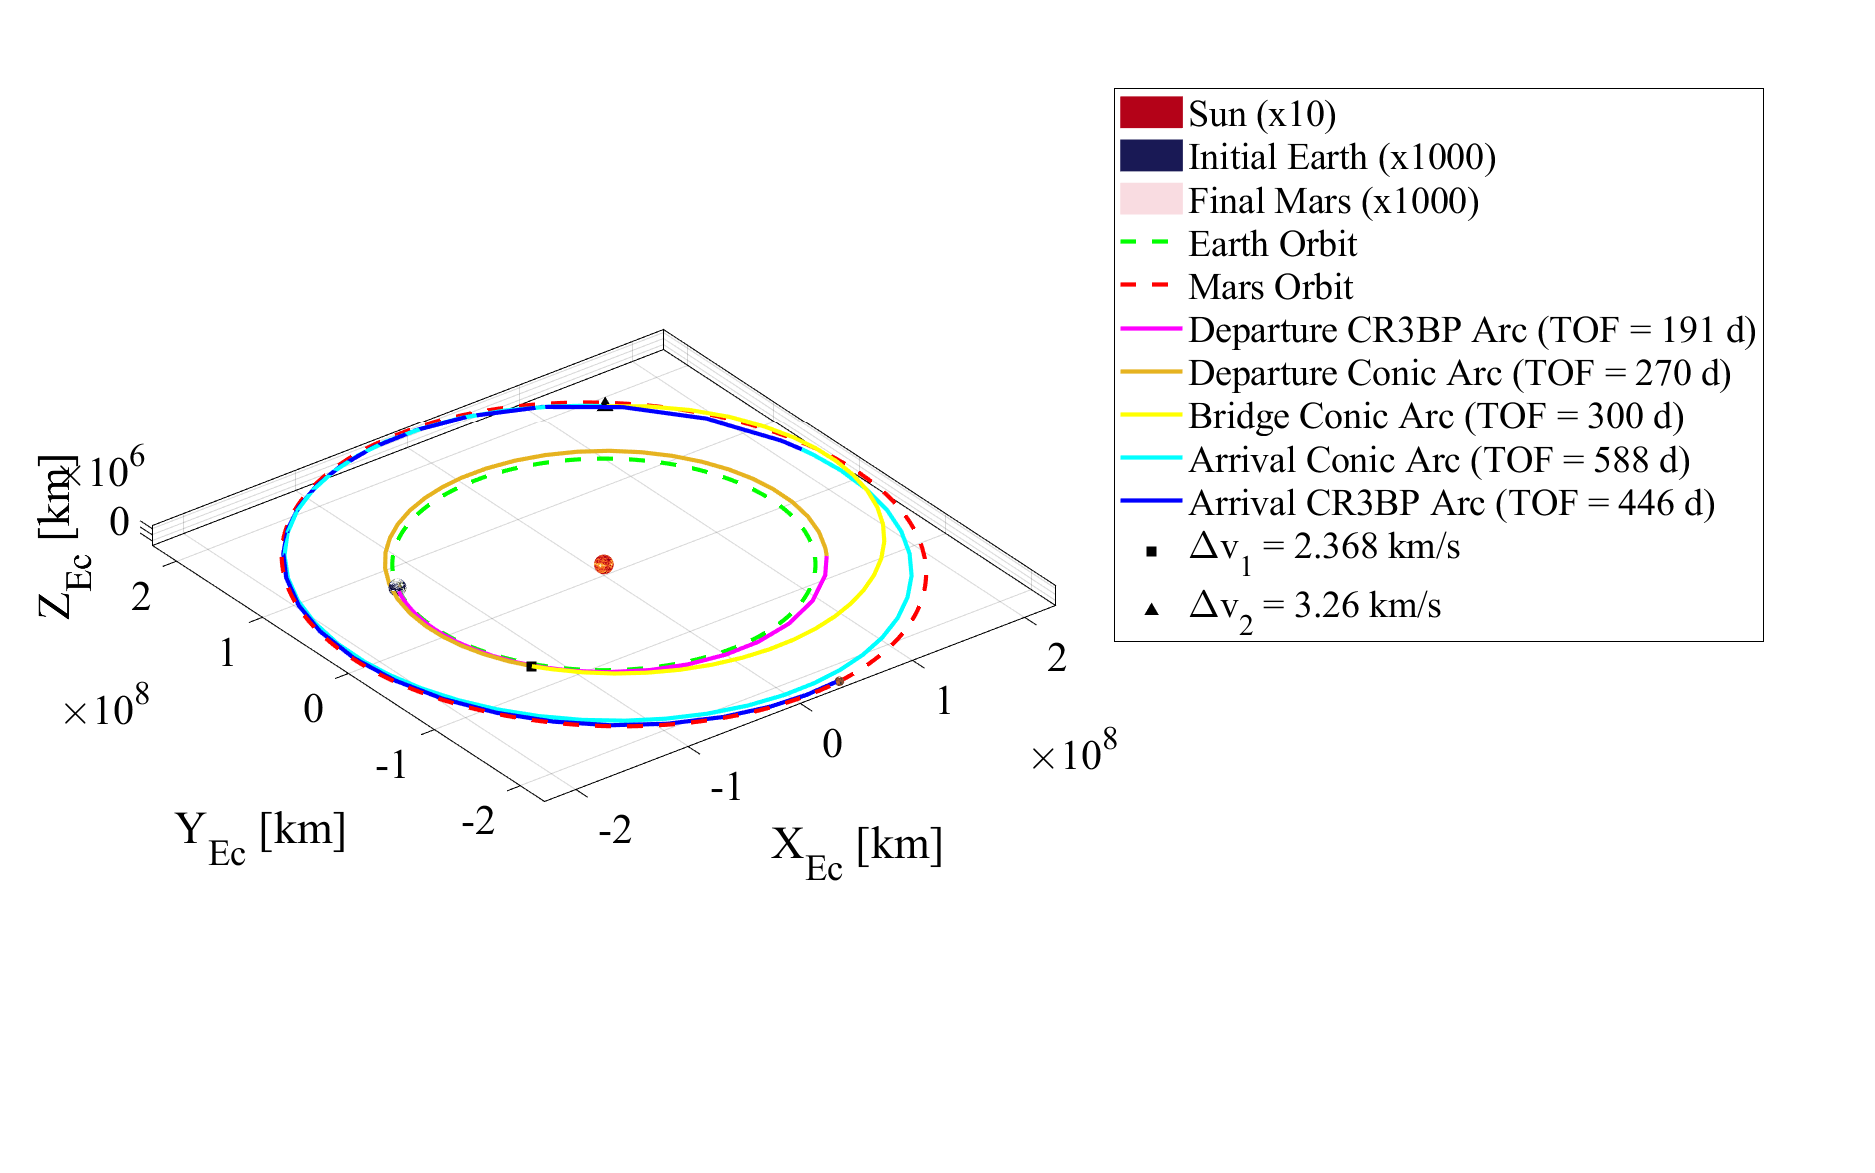
\includegraphics[width=0.9\textwidth]{figures/DirectMMAT.pdf}
    \caption{"Direct" MMAT in the Sun-centered Ecliptic J2000 frame.}
    \label{fig:directMMAT}
\end{figure}

\subsection{Transfers with an Intermediate Staging Orbit}
\begin{enumerate}
    \item   Starting from the Earth-Moon CR3BP departure orbit, a near-ballistic transfer to a
            Sun-Earth northern halo orbit is computed using the methodology introduced in Section
            4.1. The particular Sun-Earth halo is free to change to decrease the $\Delta v$ of this
            maneuver. This sets the initial epoch of the transfer.
    \item   Once in the Sun-Earth orbit, since the phase along the orbit is determined by the
            arrival onto the orbit, unstable manifold arcs of the Sun-Earth halo are propagated to
            the edge of the Earth's SoI according to the time-correspondent location along the
            orbit. Each departure CR3BP arc is then associated with a departure epoch from the
            Sun-Earth orbit.
    \item   Now similar to the "direct" transfers, these arcs serve as a departure CR3BP arc and
            departure conic arc for the MMAT methodology (Section 4.2). This produces two
            end-to-end transfers between an Earth-Moon and Sun-Mars orbit with an intermediate
            staging Sun-Earth halo orbit for each feasible manifold arc.
\end{enumerate}

\cref{fig:stagedEM}-\cref{fig:stagedMMAT} show a sample transfer with an intermediate Sun-Earth
staging halo orbit. The departure from the Earth-Moon orbit in \cref{fig:stagedEM} is similar to
the "direct" transfer example, using the same $L_{2}$ orbit. However, a different manifold arc is
used for this particular transfer. The near-ballistic transfer is shown in \cref{fig:stagedSE},
where the Earth-Moon orbit is connected to the Sun-Earth northern halo orbit. The departure CR3BP
arc is also shown leaving this orbit along the unstable manifold, which is then used in the MMAT in
\cref{fig:stagedMMAT}. Once again, this is not an optimized or minimum transfer in the family, with
a total maneuver cost of $5.481$ km/s and time-of-flight of $4.59$ years.

\begin{figure}[ht]
    \centering
    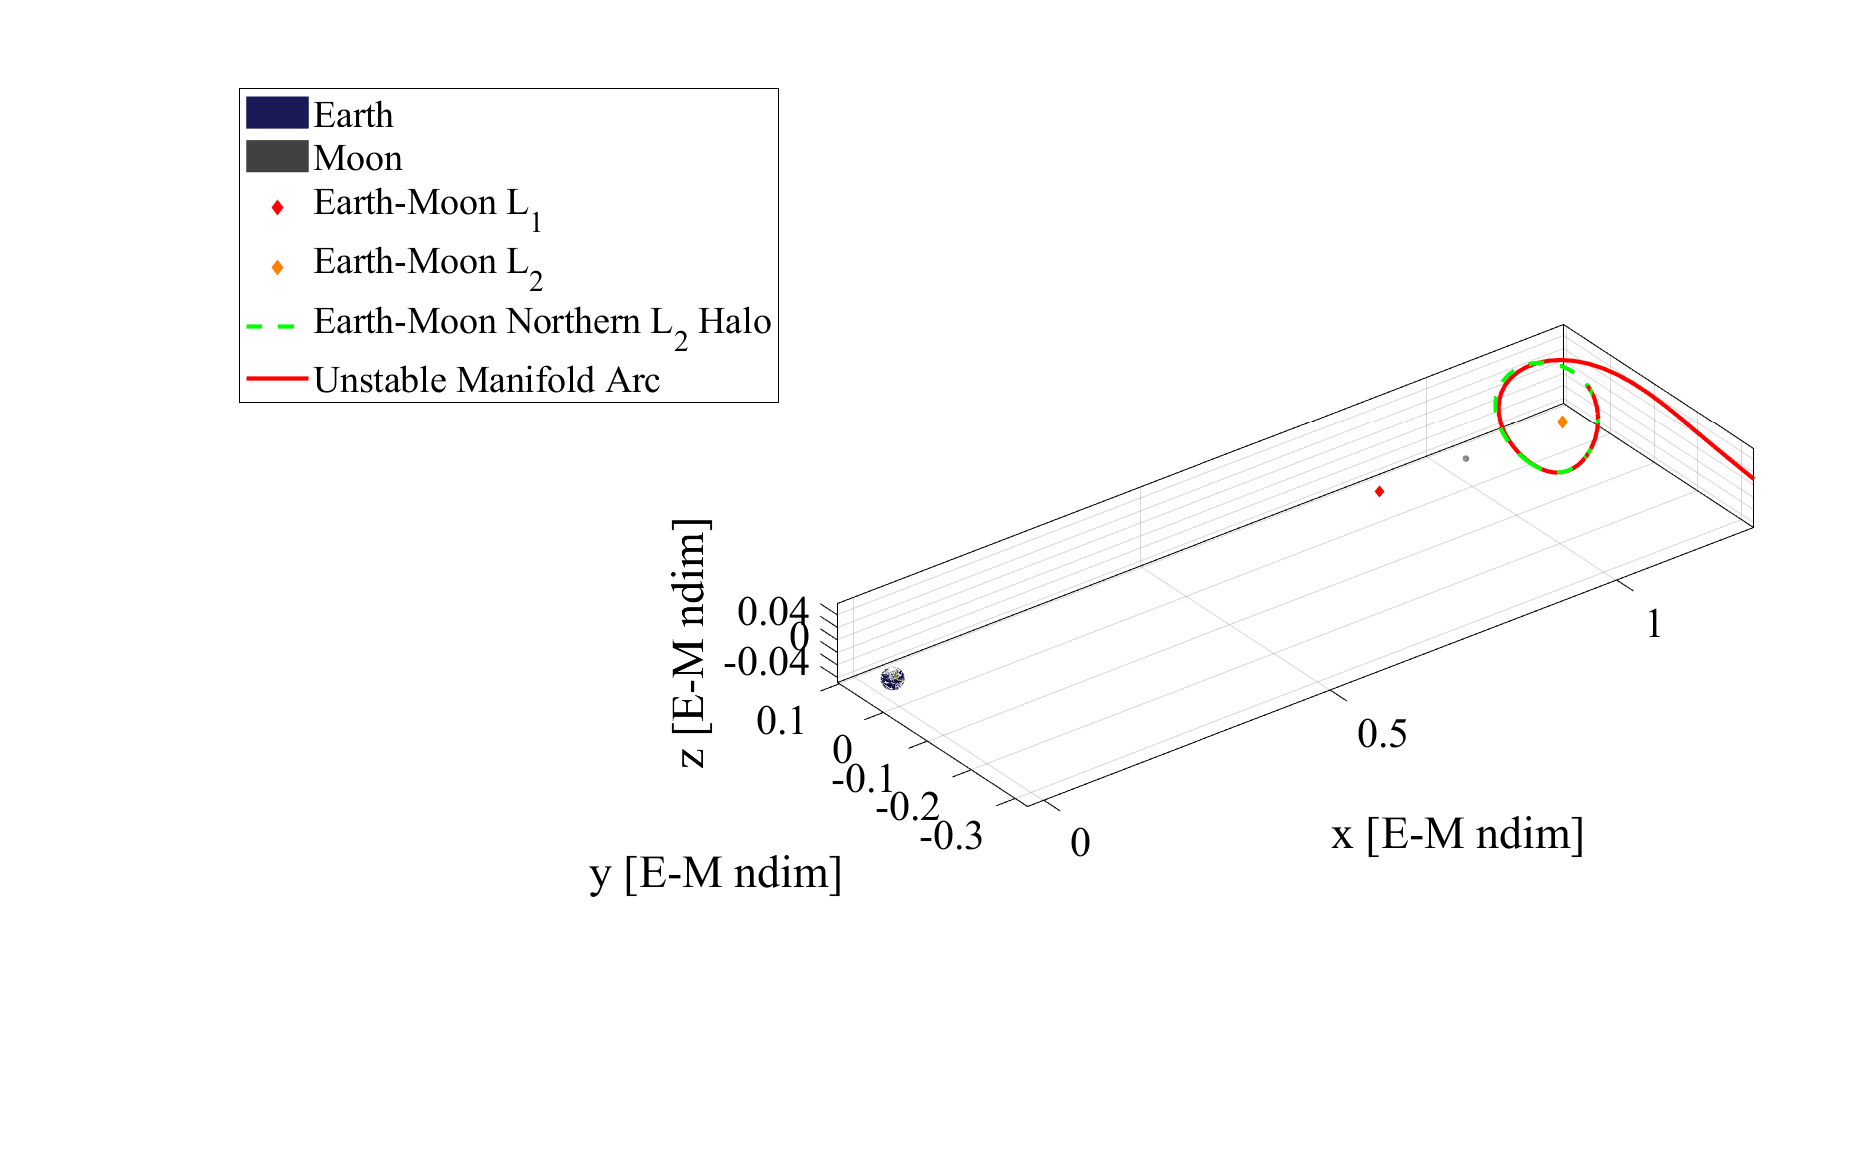
\includegraphics[width=0.9\textwidth]{figures/StagedEM.pdf}
    \caption{Departure unstable manifold arc in the Earth-Moon barycentric rotating frame.}
    \label{fig:stagedEM}
\end{figure}

\begin{figure}[ht]
    \centering
    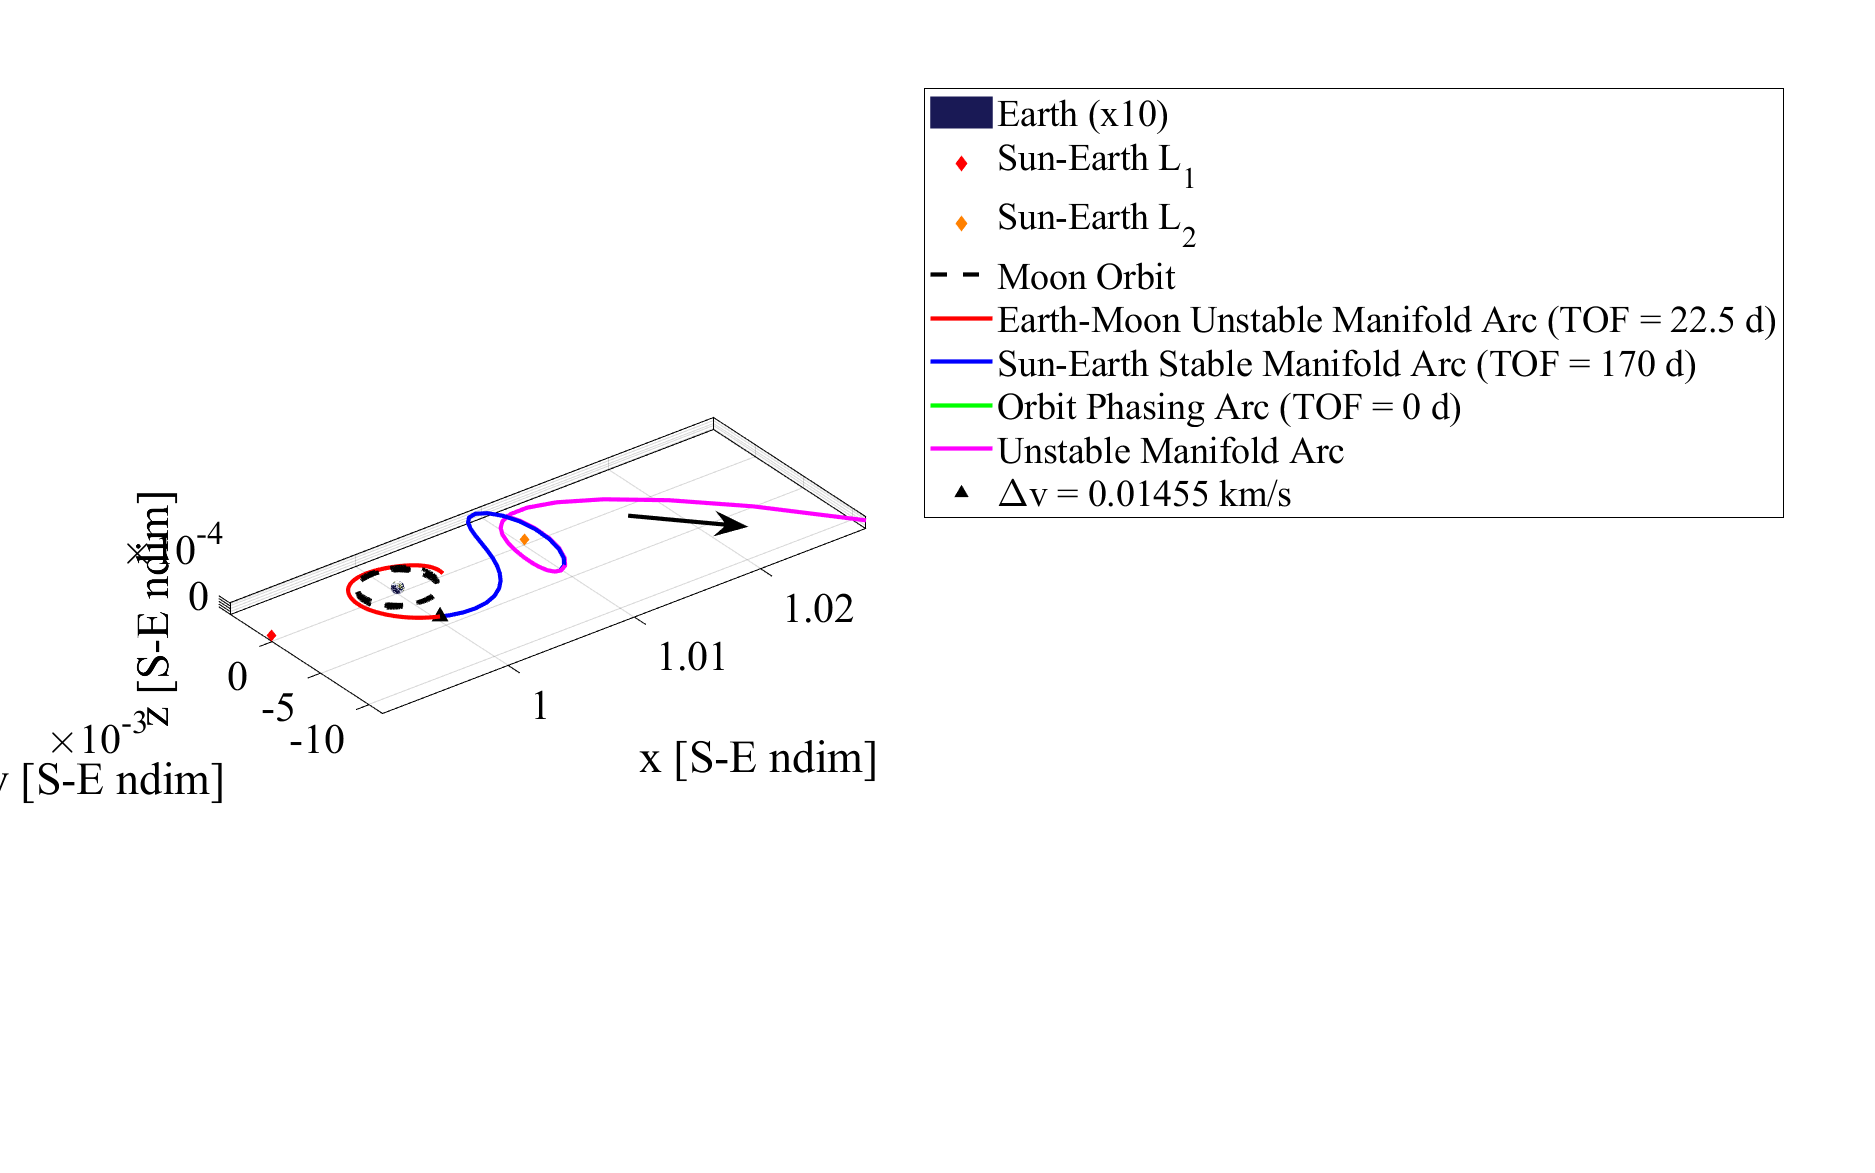
\includegraphics[width=0.9\textwidth]{figures/StagedSE.pdf}
    \caption{Departure CR3BP arc with staging orbit in the Sun-Earth barycentric rotating frame.}
    \label{fig:stagedSE}
\end{figure}

\begin{figure}[ht]
    \centering
    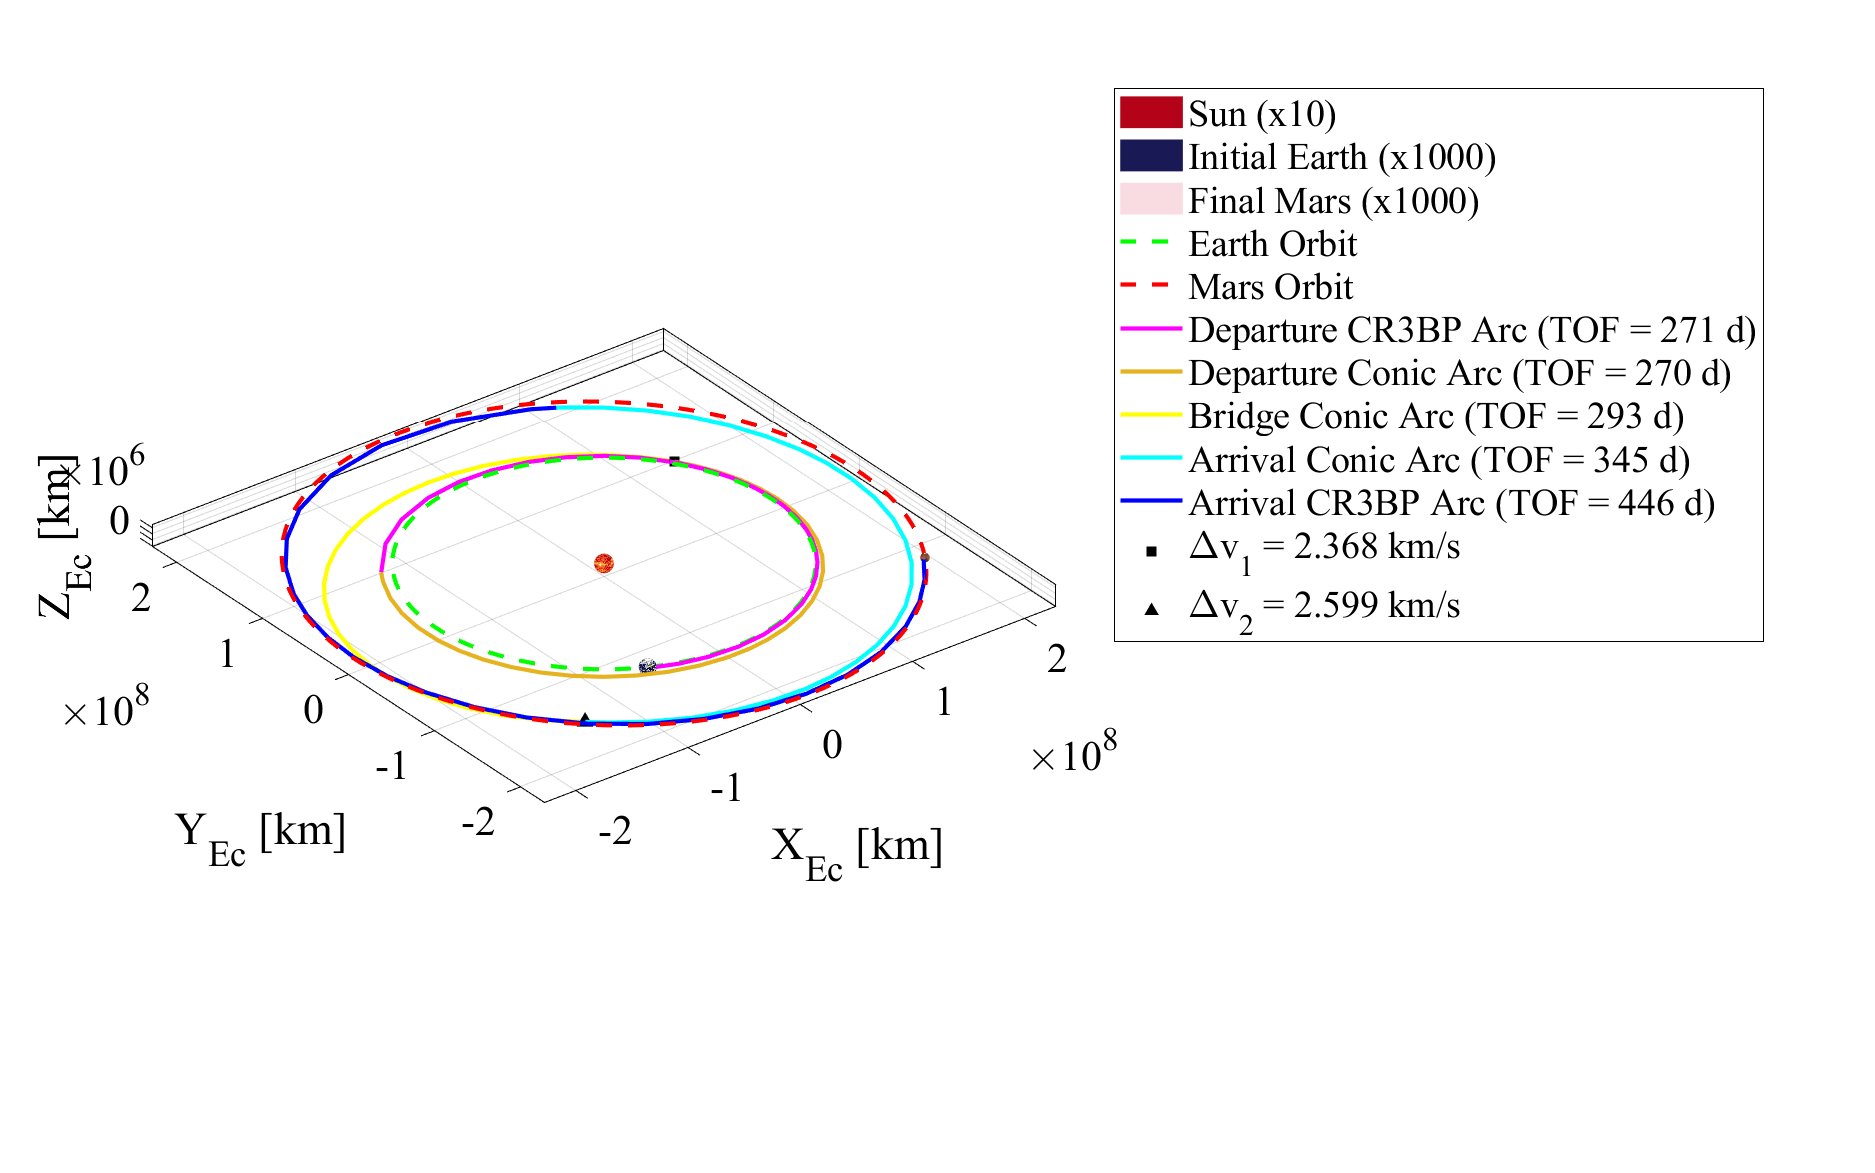
\includegraphics[width=0.9\textwidth]{figures/StagedMMAT.pdf}
    \caption{MMAT with staging orbit in the Sun-centered Ecliptic J2000 frame.}
    \label{fig:stagedMMAT}
\end{figure}

\subsection{Transfer Tradespace}
As mentioned, both categories of transfers exist in families, so the solutions will have a range of
total $\Delta v$ costs and times-of-flight. \cref{fig:tradespace} shows one such tradespace for
transfers originating from a $JC=3.13$ Earth-Moon northern $L_{2}$ halo orbit (the same used for
the previous examples). In the figure, the red points represent the family of transfers that
include a staging orbit, while the blue points represent the family of "direct" transfers. The
black "Hohmann" transfer line serves as a $\Delta v$ baseline for comparison (this will be detailed
further in the following section).

\begin{figure}[ht]
    \centering
    \includegraphics[width=0.75\textwidth]{figures/Tradespace.pdf}
    \caption{Tradespace of both solution categories originating from the same Earth-Moon departure orbit.}
    \label{fig:tradespace}
\end{figure}
